%  Encoding: UTF-8
%
% %%%%%%%%%%%%%%%%%%%%%%%%%%%%%%%%%%%%%%%%%%%%%%%%%%%%%%%%%%%%%%%%%%%%%%%%%%%% %
%  Copyright (c) 2021 I.F.F. dos SANTOS
%
%  Permission is hereby granted, free of charge, to any person obtaining a copy 
%  of this software and associated documentation files (the “Software”), to 
%  deal in the Software without restriction, including without limitation the 
%  rights to use, copy, modify, merge, publish, distribute, sublicense, and/or
%  sell copies of the Software, and to permit persons to whom the Software is 
%  furnished to do so, subject to the following conditions:
%
%  The above copyright notice and this permission notice shall be included in 
%  all copies or substantial portions of the Software.
%
%  THE SOFTWARE IS PROVIDED “AS IS”, WITHOUT WARRANTY OF ANY KIND, EXPRESS OR 
%  IMPLIED, INCLUDING BUT NOT LIMITED TO THE WARRANTIES OF MERCHANTABILITY, 
%  FITNESS FOR A PARTICULAR PURPOSE AND NONINFRINGEMENT. IN NO EVENT SHALL THE 
%  AUTHORS OR COPYRIGHT HOLDERS BE LIABLE FOR ANY CLAIM, DAMAGES OR OTHER 
%  LIABILITY, WHETHER IN AN ACTION OF CONTRACT, TORT OR OTHERWISE, ARISING 
%  FROM, OUT OF OR IN CONNECTION WITH THE SOFTWARE OR THE USE OR OTHER DEALINGS 
%  IN THE SOFTWARE.
% %%%%%%%%%%%%%%%%%%%%%%%%%%%%%%%%%%%%%%%%%%%%%%%%%%%%%%%%%%%%%%%%%%%%%%%%%%%% %
\documentclass[
   % -- opções da classe memoir --
   12pt,                         % tamanho da fonte.
   openright,                    % capítulos começam em pág ímpar (insere página vazia caso preciso).
   oneside,                      % para impressão em recto. Oposto a toweside.
   a4paper,                      % tamanho do papel. 
   sumario = tradicional,        % Para indentar os sumários
]{abntex2}

%  Encoding: UTF-8
%
% %%%%%%%%%%%%%%%%%%%%%%%%%%%%%%%%%%%%%%%%%%%%%%%%%%%%%%%%%%%%%%%%%%%%%%%%%%%% %
%  Copyright (c) 2021 I.F.F. dos SANTOS
%
%  Permission is hereby granted, free of charge, to any person obtaining a copy 
%  of this software and associated documentation files (the “Software”), to 
%  deal in the Software without restriction, including without limitation the 
%  rights to use, copy, modify, merge, publish, distribute, sublicense, and/or
%  sell copies of the Software, and to permit persons to whom the Software is 
%  furnished to do so, subject to the following conditions:
%
%  The above copyright notice and this permission notice shall be included in 
%  all copies or substantial portions of the Software.
%
%  THE SOFTWARE IS PROVIDED “AS IS”, WITHOUT WARRANTY OF ANY KIND, EXPRESS OR 
%  IMPLIED, INCLUDING BUT NOT LIMITED TO THE WARRANTIES OF MERCHANTABILITY, 
%  FITNESS FOR A PARTICULAR PURPOSE AND NONINFRINGEMENT. IN NO EVENT SHALL THE 
%  AUTHORS OR COPYRIGHT HOLDERS BE LIABLE FOR ANY CLAIM, DAMAGES OR OTHER 
%  LIABILITY, WHETHER IN AN ACTION OF CONTRACT, TORT OR OTHERWISE, ARISING 
%  FROM, OUT OF OR IN CONNECTION WITH THE SOFTWARE OR THE USE OR OTHER DEALINGS 
%  IN THE SOFTWARE.
% %%%%%%%%%%%%%%%%%%%%%%%%%%%%%%%%%%%%%%%%%%%%%%%%%%%%%%%%%%%%%%%%%%%%%%%%%%%% %


% --------------------------------------
% Aparência
% --------------------------------------

\usepackage[T1]{fontenc}               % Compilar correctamente com pdflatex
\usepackage[utf8x]{inputenc}           % Codificacao do documento (conversão automática dos acentos).
\usepackage{ucs}                       % Complemento do anterior.
\usepackage{indentfirst}               % Indenta o primeiro parágrafo

\PassOptionsToPackage{
   english,             % idioma adicional para hifenização.
   french,              % idioma adicional para hifenização.
   spanish,             % idioma adicional para hifenização.
   main=portuguese      % Idioma do documento
}{babel}

% 1ex - É a largura da letra x (minúscula)
% 1em - É a largura da letra M (Maiúscula)
\setlength{\parindent}{3ex}  % Tamanho 
\setlength{\parskip}{1em}    % Tamaño del parágrafo

% Margens da página
\usepackage{geometry}                          % Permite configurar as margens da página.
\geometry{hmargin={3cm,2cm},vmargin={3cm,2cm}} % Margens conforme padrão ABNT

% Pacote de citações
\usepackage[num,overcite]{abntex2cite} % Citações padrão ABNT, em ordem alfabética.
\citebrackets[]                        % Citações com coxetes.
\usepackage{bibentry}                  %

% Usar font 'TeX Gyre Termes'
\usepackage{tgtermes}

\usepackage{titlesec,titletoc}

\titleformat{\chapter}[hang]{\large\bfseries}{\thechapter. }{0pt}{\large\bfseries}
\titleformat{\section}[hang]{\normalfont\bfseries}{\thesection. }{0pt}{\normalfont\bfseries}

% --------------------------------------
% ETC
% --------------------------------------

\usepackage{graphicx}                  % Inclusão de figuras.
\usepackage{wrapfig}                   % Figuras junto com o texto
\usepackage{float}                     % Para posicionar figuras corretamente.
\usepackage{subcaption}                % Para legendas nas subfiguras.

\usepackage{amssymb}                   % Para exibir símbolos de conjuntos de números (reais, etc...).
\usepackage{amsmath}                   % Para adcionar equações
\usepackage{amsfonts}                  % Fontes para notação matemática. de cada seção.
\usepackage{esint}                     % various fancy integral symbols


\usepackage{microtype}                 % para melhorias de justificação.
\usepackage{fancyhdr}                  % Pemite alterações no cabeçalho e rodapé.
\usepackage{hyperref}                  % Cria formatação automática de PDF.
\usepackage[hyphenbreaks]{breakurl}    % Quebra de linha em url.
\usepackage{lettrine}				      % letras capitulares

\usepackage[htt]{hyphenat}  % Permitir hifenização usando \texttt

\usepackage{enumitem}

% --------------------------------------
% Para notación formal de proposiciónes
% --------------------------------------
\usepackage{amsthm, thmtools}

\declaretheoremstyle[
   headfont=\normalfont\bfseries,
   bodyfont=\normalfont\itshape,
   notefont=\normalfont\bfseries,
   notebraces={ (}{)},
   headpunct={. },
   numbered=yes,
   spaceabove=1em,
   postheadspace=0em,
   spacebelow=1em,
   qed={ }
]{EstiloItalico}
\declaretheoremstyle[
   headfont=\normalfont\bfseries,
   bodyfont=\normalfont\mdseries,
   notefont=\normalfont\bfseries,
   notebraces={ (}{)},
   headpunct={. },
   numbered=yes,
   spaceabove=1em,
   postheadspace=0em,
   spacebelow=1em,
   qed={ }
]{EstiloPlano}

% Lei
\declaretheorem[
   style=EstiloItalico,
   parent=chapter,
   name=Lei
]{lei}

% Axiomas
\declaretheorem[
   style=EstiloItalico,
   parent=chapter,
   name=Axioma
]{axioma}

% Postulados
\declaretheorem[
   style=EstiloItalico,
   parent=chapter,
   name=Postulado
]{postulado}

% Definição
\declaretheorem[
   style=EstiloPlano,
   parent=chapter,
   name=Defini\c{c}\~ao
]{definicao}

% Teorema
\declaretheorem[
   style=EstiloItalico,
   parent=chapter,
   name=Teorema
]{teorema}

% Prova
\declaretheorem[
   style=EstiloPlano,
   numbered=no,
   qed={C.Q.D.},
   name=Desmostra\c{c}\~ao
]{prova}

% Exemplo
\declaretheorem[
   style=EstiloPlano,
   parent=chapter,
   name=Exemplo
]{exemplo}

% Pergunta
\declaretheorem[
   style=EstiloItalico,
   name=Pergunta
]{pergunta}

% --------------------------------------
% Para exibição de código fonte
% --------------------------------------

% see https://en.wikibooks.org/wiki/LaTeX/Source_Code_Listings

\usepackage{listings}
\usepackage{xcolor}

% see https://latexcolor.com/
\definecolor{codegreen}{rgb}{0,0.6,0}
\definecolor{codegray}{rgb}{0.5,0.5,0.5}
\definecolor{amaranth}{rgb}{0.9, 0.17, 0.31}

\usepackage{caption}
\DeclareCaptionFont{white}{\color{white}}
\DeclareCaptionFormat{listing}{\hspace*{-0.4pt}\colorbox{gray}{\parbox{\textwidth}{#1#2#3}}}
\captionsetup[lstlisting]{format=listing,labelfont=white,textfont=white}

\renewcommand{\lstlistingname}{Código}

\lstset{
   backgroundcolor=\color{white},   % choose the background color; you must add \usepackage{color} or \usepackage{xcolor}; should come as last argument
   basicstyle=\mdseries\ttfamily\scriptsize, % the size of the fonts that are used for the code
   breakatwhitespace=false,         % sets if automatic breaks should only happen at whitespace
   breaklines=true,                 % sets automatic line breaking
   captionpos=t,                    % sets the caption-position to bottom
   columns=fixed,                   % Using fixed column width (for e.g. nice alignment)
   escapechar=µ,
   numbers=none,                    % Not use numbers
   frame=single,	                  % adds a frame around the code
   keepspaces=true,                 % keeps spaces in text, useful for keeping indentation of code (possibly needs columns=flexible)
   rulecolor=\color{black},         % if not set, the frame-color may be changed on line-breaks within not-black text (e.g. comments (green here))
   showspaces=false,                % show spaces everywhere adding particular underscores; it overrides 'showstringspaces'
   showstringspaces=false,          % underline spaces within strings only
   showtabs=false,                  % show tabs within strings adding particular underscores
   tabsize=3  	                     % sets default tabsize to 3 spaces
}

\lstdefinestyle{c}{
   language=C, % the language of the code (can be overrided per snippet)
   commentstyle=\color{codegray}, % comment style
   keywordstyle={\color{codegreen}\bfseries},
   stringstyle=\color{amaranth} % string literal style
}

\lstdefinestyle{f90}{
   language=Fortran, % the language of the code (can be overrided per snippet)
   commentstyle=\color{codegray}, % comment style
   keywordstyle={\color{codegreen}\bfseries},
   stringstyle=\color{amaranth} % string literal style
}

\lstdefinestyle{java}{
   language=Java, % the language of the code (can be overrided per snippet)
   commentstyle=\color{codegray}, % comment style
   keywordstyle={\color{codegreen}\bfseries},
   stringstyle=\color{amaranth} % string literal style
}

\lstdefinestyle{py}{
   language=Python, % the language of the code (can be overrided per snippet)
   commentstyle=\color{codegray}, % comment style
   keywordstyle={\color{codegreen}\bfseries},
   stringstyle=\color{amaranth} % string literal style
}

\lstdefinestyle{gnuplot}{
   language=Gnuplot, % the language of the code (can be overrided per snippet)
   commentstyle=\color{codegray}, % comment style
   keywordstyle={\color{codegreen}\bfseries},
   stringstyle=\color{amaranth} % string literal style
}

\lstdefinestyle{bash}{
   language=bash, % the language of the code (can be overrided per snippet)
   commentstyle=\color{codegray}, % comment style
   keywordstyle={\color{codegreen}\bfseries},
   stringstyle=\color{amaranth}, % string literal style
   morekeywords={apt, pacman, yum, zypper, dnf, dns, mkdir, cp, configure, make, tar},
}

\lstdefinestyle{pseudo}{
   commentstyle=\color{codegray}, % comment style
   keywordstyle={\color{codegreen}},
   stringstyle=\color{amaranth}, % string literal style
   morekeywords={inicio, fim, para, ate, subrotinas, se, senao, entao, funcao, inteiro, enquanto, gnuplot, logico, verdadeiro, subrotina, variavel},
   morestring=[b]",
   morecomment={[l]//},
   inputencoding=utf8,
   extendedchars=true,
   literate=%
      {á}{{\'a}}1 {é}{{\'e}}1 {í}{{\'i}}1 {ó}{{\'o}}1 {ú}{{\'u}}1
      {Á}{{\'A}}1 {É}{{\'E}}1 {Í}{{\'I}}1 {Ó}{{\'O}}1 {Ú}{{\'U}}1
      {à}{{\`a}}1 {è}{{\`e}}1 {ì}{{\`i}}1 {ò}{{\`o}}1 {ù}{{\`u}}1
      {À}{{\`A}}1 {È}{{\'E}}1 {Ì}{{\`I}}1 {Ò}{{\`O}}1 {Ù}{{\`U}}1
      {ä}{{\"a}}1 {ë}{{\"e}}1 {ï}{{\"i}}1 {ö}{{\"o}}1 {ü}{{\"u}}1
      {Ä}{{\"A}}1 {Ë}{{\"E}}1 {Ï}{{\"I}}1 {Ö}{{\"O}}1 {Ü}{{\"U}}1
      {â}{{\^a}}1 {ê}{{\^e}}1 {î}{{\^i}}1 {ô}{{\^o}}1 {û}{{\^u}}1
      {Â}{{\^A}}1 {Ê}{{\^E}}1 {Î}{{\^I}}1 {Ô}{{\^O}}1 {Û}{{\^U}}1
      {ã}{{\~a}}1 {ẽ}{{\~e}}1 {ĩ}{{\~i}}1 {õ}{{\~o}}1 {ũ}{{\~u}}1
      {Ã}{{\~A}}1 {Ẽ}{{\~E}}1 {Ĩ}{{\~I}}1 {Õ}{{\~O}}1 {Ũ}{{\~U}}1
      {œ}{{\oe}}1 {Œ}{{\OE}}1 {æ}{{\ae}}1 {Æ}{{\AE}}1 {ß}{{\ss}}1
      {ű}{{\H{u}}}1 {Ű}{{\H{U}}}1 {ő}{{\H{o}}}1 {Ő}{{\H{O}}}1
      {ç}{{\c c}}1 {Ç}{{\c C}}1 {ø}{{\o}}1 {å}{{\r a}}1 {Å}{{\r A}}1
      {€}{{\euro}}1 {£}{{\pounds}}1 {«}{{\guillemotleft}}1
      {»}{{\guillemotright}}1 {ñ}{{\~n}}1 {Ñ}{{\~N}}1 {¿}{{?`}}1 {¡}{{!`}}1
      {←}{{$\leftarrow$}}1
      {!=}{{$\neq$}}1
}

% --------------------------------------
% Para fluxogramas
% --------------------------------------

\usepackage{tikz}

\usetikzlibrary{shapes.geometric, arrows}
\tikzstyle{startstop} = [rectangle, rounded corners, minimum width=3cm, minimum height=1cm,text centered, draw=black]
\tikzstyle{io} = [trapezium, trapezium left angle=70, trapezium right angle=110, minimum width=3cm, minimum height=1cm, text centered, draw=black]
\tikzstyle{process} = [rectangle, minimum width=3cm, minimum height=1cm, text centered, draw=black]
\tikzstyle{decision} = [diamond, minimum width=3cm, minimum height=1cm, text centered, draw=black]
\tikzstyle{conector} = [circle, minimum width=0.5cm, minimum height=0.5cm, text centered, draw=black]
\tikzstyle{arrow} = [thick,->,>=stealth]
\tikzstyle{line} = [draw, -latex']

% --------------------------------------
% CONFIGURAÇÕES DE PACOTES
% --------------------------------------
\newcommand{\cqd}{C.Q.D.}

\newcommand{\R}{\mathbb{R}}
\newcommand{\C}{\mathbb{C}}
\newcommand{\Z}{\mathbb{Z}}
\newcommand{\N}{\mathbb{N}}
\newcommand{\E}{\mathbb{E}}
\newcommand{\M}{\mathbb{M}}

\newcommand{\F}{\mathcal{F}}

\newcommand{\sen}{\operatorname{sen}}
\newcommand{\asen}{\,\operatorname{arcsen}\,}

\newcommand{\bra}[1]{\langle#1|}
\newcommand{\ket}[1]{|#1\rangle}
\newcommand{\braket}[2]{\langle#1|#2\rangle}
\newcommand{\ketbra}[2]{|#1\rangle\langle#2|}

\newcommand{\eq}[1]{\hyperref[eq:#1]{equa\c{c}\~ao} \ref{eq:#1}}

\newcommand{\aspas}[1]{``#1''}

\newcommand{\gnuplot}{\ttfamily gnuplot \rmfamily }


\makeatletter
\titulo{ % Não aceita ascento
   Introdu\c{c}\~ao \`a F\'isica Computacional
}
\autor{I. F. F. dos SANTOS}
\local{Maceió} % Aceita ascento
\data{\today}
\makeatother

\hypersetup{
   %pagebackref=true,
   pdftitle={Introdu\c{c}\~ao \`a F\'isica Computacional}, 
   pdfauthor={\imprimirautor},
   pdfcreator={LaTeX with abnTeX2},
   pdfkeywords={Física},
   %pagebackref=true,
   bookmarksdepth=4,
   % Caso o documento seja impresso, marque a opção abaixo como false,
   % caso contrário, recomendo que matenha como true.
   colorlinks=true,            % false: boxed links; true: colored links
   linkcolor=blue,             % color of internal links
   citecolor=blue,             % color of links to bibliography
   filecolor=mageta,           % color of file links
   urlcolor=blue
}

\begin{document}
\nobibliography{reference}
% ------------------------------------------------------------------------------
% ELEMENTOS PRÉ-TEXTUAIS
% ------------------------------------------------------------------------------
   ~
\vspace{5em}
\hrule
\begin{center}
   \huge
   \imprimirtitulo \\
   \normalsize
   \imprimirautor
   \hfill
   \imprimirlocal, \imprimirdata
\end{center}
\hrule

   \newpage
\hrule
\begin{center}
   \huge
   \imprimirtitulo \\
   \normalsize
   \imprimirautor
   \hfill
   Versão 1.1
\end{center}
\hrule
\vfill
\begin{center}
Esta apostila foi escrita usando \LaTeX.\\
O código fonte pode ser encontrado em\\
\url{https://github.com/ismaeldamiao/Apostila_de_IFC}
\end{center}
\newpage

% ---
% SUMÁRIOS
% ---
   \pdfbookmark[0]{\contentsname}{toc}
   \tableofcontents*
   \pagebreak
% ------------------------------------------------------------------------------
% ELEMENTOS TEXTUAIS
% ------------------------------------------------------------------------------
   \textual
   % %%%%%%%%%%%%%%%%%%%%%%%%%%%%%%%%%%%%%%%%%%%%%%%%%%%%%%%%%%%%%%%%%%%%%%%%%%%%%%
% Introdução
% %%%%%%%%%%%%%%%%%%%%%%%%%%%%%%%%%%%%%%%%%%%%%%%%%%%%%%%%%%%%%%%%%%%%%%%%%%%%%%
\chapter{Introdução}

\lettrine{Q}{uando} queremos dividir a física em ramos, para facilitar a
sua compreensão, geralmente pensamos em dois principais ramos,
a saber, Física Teórica e Física Experimental; Você deve ter estudado um pouco sobre
ambos mas há ainda outro ramo que não pode ser encaixado nesses dois e é
a Física Computacional, ela por sua vez pode ser organizada em outros
quatro ramos 1) modelagem: Tanto a Física Teórica
quanto a Computacional usam modelagem,
os físicos buscam descrever os fenômenos da natureza utilizando modelagem matemática.
2) Instrumentação: Tanto a Física Experimental quanto a Computacional
buscam desenvolver e utilizar equipamentos sofisticados, o que inclui aparatos de
alto custo e criação de novas tecnologias, acontece que os
experimentais usam os equipamentos para medir, ou seja para saber o que acontece
quando a natureza interage com o aparato e daí fazer a coleta de dados enquanto
que os computacionais usam esses recursos para implementar algoritmos de computador.
3) Tratamento de dados: Tanto a Física Experimental quanto a Computacional
realizam coleta de dados e se faz necessário o uso de diversos meios
para análise e interpretação desse dados. 4) Simulação:
Especialidade da Física Computacional, uma vez que se possui um modelo teórico
então chega o momento de simular um experimento físico.

Uma simulação é como um mini universo cujo as leis da física
são justamente as do modelo teórico, é a simulação de um experimento que
produz os dados a serem analisados mas, diferente da Física Experimental que
quer verificar se a natureza de fato obedece o modelo, na Física
Computacional o modelo sempre é obedecido pela simulação (exceto em erros de
programação) o que é uma diferença notável. Apesar de que a metodologia
de simulação lembra a de experimentação e de que a análise de dados
de um experimento e de uma simulação segue basicamente os mesmos princípios,
as conclusões que uma simulação fornece não têm tanta importância quanto
as conclusões que um experimento fornece, tal importância continua no patamar
especulativo, característica comum entre os trabalhos teóricos.

Os conhecimentos obtidos no estudo da computação lhe permitirão
resolver equações algébricas e diferenciais, calcular derivadas e integrais,
realizar transformadas de Fourrier e Laplace, fazer análise estatística de dados,
etc, além de lhe proporcionar base para outras atividades como escrever
documentos em \LaTeX, escrever scripts para melhor gerenciamento do seu computador,
etc.

O objetivo deste nivelamento é incentivar a estudar a programação
antes mesmo de se deparar com as matérias a isso dedicadas, assim o choque
não será tão grande quando chegar na matéria.

Neste módulo introdutório iremos
aprender sobre algoritmos, pseudocódigos e fluxogramas,
fazer uma introdução à linguagens
de programação,
conhecer o programa \textit{Ola Mundo} de algumas
linguagens e ver algumas aplicações básicas da programação
para os primeiros períodos do curso de física.

% %%%%%%%%%%%%%%%%%%%%%%%%%%%%%%%%%%%%%%%%%%%%%%%%%%%%%%%%%%%%%%%%%%%%%%%%%%%%%%
% Prelúdio aos Algoritmos
% %%%%%%%%%%%%%%%%%%%%%%%%%%%%%%%%%%%%%%%%%%%%%%%%%%%%%%%%%%%%%%%%%%%%%%%%%%%%%%
\chapter{Prelúdio aos Algoritmos}

\lettrine{``C}{omo} você os ensina alguma coisa nova? Misturando o que
eles sabem com o que eles não sabem'' já dizia Picasso e é justamente
essa a filosofia de um algoritmo, um algoritmo é uma série de instruções
sobre como fazer alguma coisa e essas instruções devem estar divididas
em pequenas partes simples que, quando seguidas todas, levam a execução
de uma tarefa complexa.

Por exemplo, calcular o fatorial de um número natural não é uma tarefa simples
pois está além das quatro operações básicas e se você quiser ensinar alguém
a calcular o fatorial então deverá dividir essa tarefa em outras tarefas mais
simples. Comece por observar a definição do fatorial.

\[
n! = n \cdot (n-1)! = \prod_{i=1}^{n} i = 1 \cdot 2 \cdot ... \cdot n ~\forall~n\in\Z
\]

Foque na parte $n! = \prod_{i=1}^{n} i$, uma série de instruções simples para
calcular o fatorial de $n$ seriam:
\begin{enumerate}[nosep]
\item Calcule $1\cdot 2$.
\item $n = 2$? Se sim então $n! = 1\cdot 2$. Senão então calcule $x_3 = 2 \cdot 3$.
\item $n = 3$? Se sim então $n! = x_3$. Senão então calcule $x_4 = x_3 \cdot 4$.
\item $n = 4$? Se sim então $n! = x_4$. Senão então calcule $x_5 = x_4 \cdot 5$.
\item $...$
\item $n = x_i$? Se sim então $n! = x_i$. Senão então calcule $x_{i+1} = x_i \cdot (i+1)$.
\end{enumerate}

Por outro lado, da parte $n! = n\cdot(n-1)!$ vem um algoritmo mais simples.
\begin{enumerate}[nosep]
\item $n=1$? Se sim então $n!=1$. Senão então calcule $n \cdot (n-1)!$
\end{enumerate}

\noindent
Nesse último caso fica a pergunta: Como calcular $(n-1)!$? mas a resposta
é simples, basta começar o algoritmo de novo e testar se $(n-1)=1$, ou seja,
o algoritmo é autorreferente, se o procedimento ainda não é o suficiente simples
então você deve começar novamente o algoritmo, e novamente... até que o procedimento
seja suficientemente simples. Este tipo de algoritmo é chamado \textbf{recursivo},
enquanto que o tipo anterior é chamado \textbf{iterativo}, obviamente há outros tipos de algoritmos.

Há duas principais maneiras de representar algoritmos, a saber, usando
pseudocódigo ou fluxogramas. Vejamos como as usar.

\section{Fluxograma}

Um fluxograma é uma figura que exemplifica um algoritmo de forma simples
e intuitiva. Por exemplo, o fluxograma abaixo mostra como calcular o
fatorial de um número.

\begin{figure}[H]
   \centering
   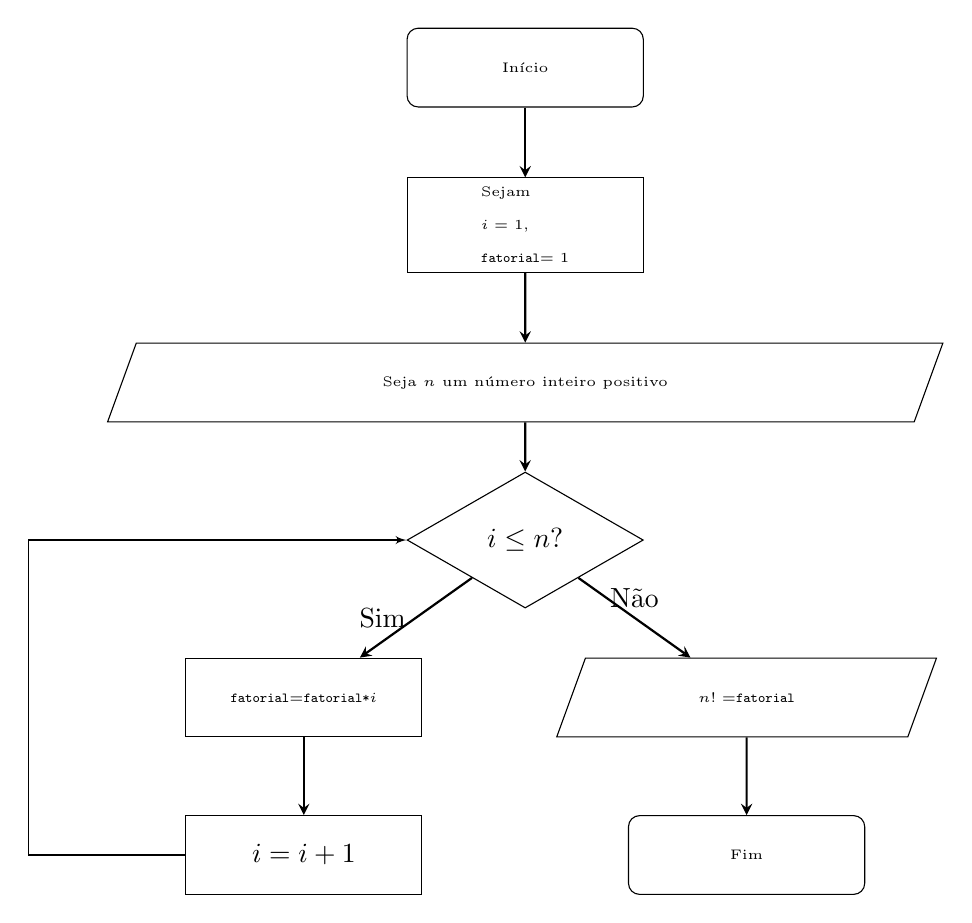
\begin{tikzpicture}[node distance=2cm]

   \node (start) [startstop] {\tiny Início};
   \node (decl) [process, below of=start, align=left] {\tiny Sejam\\\tiny $i=1$,\\\tiny \texttt{fatorial}$=1$};
   \node (in) [io, below of=decl, align=left] {\tiny Seja $n$ um número inteiro positivo};

   \node (for) [decision, below of=in] {$i \leq n$?};
   \node (calc) [process, below of=for, xshift=-8em] {\tiny \texttt{fatorial}$=$\texttt{fatorial*}$i$};
   \node (ii) [process, below of=calc] {$i=i+1$};

   \node (result) [io, below of=for, xshift=8em] {\tiny $n!=$\texttt{fatorial}};

   \node (stop) [startstop, below of=result] {\tiny Fim};

   \draw [arrow] (start) -- (decl);
   \draw [arrow] (decl) -- (in);
   \draw [arrow] (in) -- (for);
   \draw [arrow] (for) -- node[anchor=east] {Sim} (calc);
   \draw [arrow] (result) -- (stop);
   \draw [arrow] (for) -- node[anchor=south] {N\~ao} (result);
   \draw [arrow] (calc) -- (ii);
   \path [line] (ii) -- ++(-3.5,0) |- (for);
   \end{tikzpicture}
\end{figure}

\begin{pergunta}
Há dois cálculos desnecessários nesse algoritmo.
Você consegue identificá-los? Como o algoritmo pode ser melhorado?
\end{pergunta}

No fluxograma há alguns símbolos mas não é preciso conhecer os símbolos para o
entender pois ele é bastante intuitivo. Basicamente, os elementos de um
fluxograma são

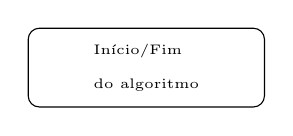
\begin{tikzpicture}
\node (null) [startstop, align=left] {\tiny Início/Fim \\\tiny do algoritmo};
\end{tikzpicture}
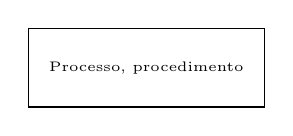
\begin{tikzpicture}
\node (null) [process, align=left] {\tiny Processo, procedimento};
\end{tikzpicture}\\
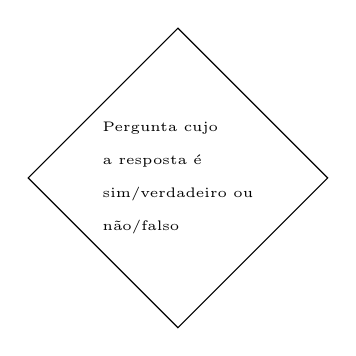
\begin{tikzpicture}
\node (null) [decision, align=left] {\tiny Pergunta cujo \\\tiny a resposta é\\\tiny sim/verdadeiro ou\\\tiny não/falso};
\end{tikzpicture}
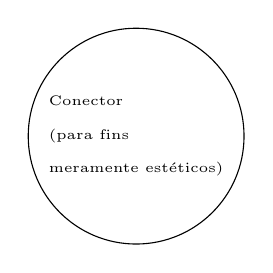
\begin{tikzpicture}
\node (null) [conector, align=left] {\tiny Conector\\\tiny (para fins\\\tiny meramente estéticos)};
\end{tikzpicture}\\
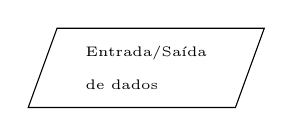
\begin{tikzpicture}
\node (null) [io, align=left] {\tiny Entrada/Saída\\\tiny de dados};
\end{tikzpicture}


\section{Pseudocódigo}

Para explicar pseudocódigo irei recorrer à sua inteligência e aos
fluxogramas.

\begin{center} Programa \end{center}
\begin{minipage}[b]{0.45\linewidth}\centering
   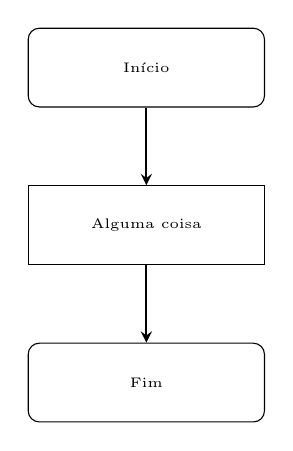
\begin{tikzpicture}[node distance=2cm]
   \node (start) [startstop] {\tiny Início};
   \node (proc) [process, below of=start] {\tiny Alguma coisa};
   \node (stop) [startstop, below of=proc] {\tiny Fim};
   \draw [arrow] (start) -- (proc);
   \draw [arrow] (proc) -- (stop);
   \end{tikzpicture}
\end{minipage}
\begin{minipage}[b]{0.45\linewidth}\centering
\begin{lstlisting}[style=pseudo]
inicio

alguma_coisa()

fim
\end{lstlisting}
\end{minipage}




\begin{center} Decisão \end{center}
\begin{minipage}[b]{0.45\linewidth}\centering
   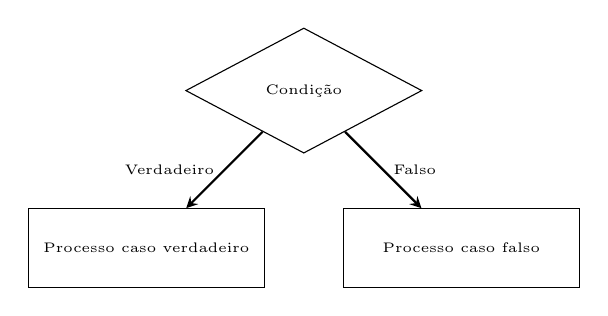
\begin{tikzpicture}[node distance=2cm]
   \node (d) [decision] {\tiny Condição};
   \node (t) [process, below of=d, xshift=-2cm] {\tiny Processo caso verdadeiro};
   \node (f) [process, below of=d, xshift=2cm] {\tiny Processo caso falso};
   \draw [arrow] (d) -- node[anchor=east] {\tiny Verdadeiro} (t);
   \draw [arrow] (d) -- node[anchor=west] {\tiny Falso} (f);
   \end{tikzpicture}
\end{minipage}
\begin{minipage}[b]{0.45\linewidth}\centering
\begin{lstlisting}[style=pseudo]
se condição entao
   Processo_caso_verdadeiro()
senao
   Processo_caso_falso()
fim se
\end{lstlisting}
\end{minipage}




\begin{center} Ciclo \aspas{Enquanto} \end{center}
\begin{minipage}[b]{0.45\linewidth}\centering
   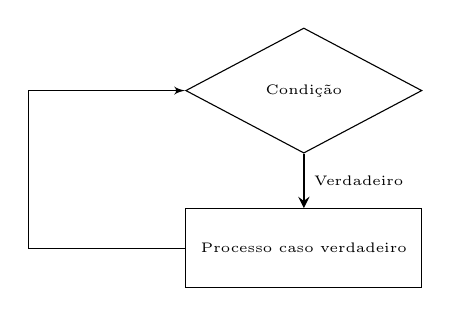
\begin{tikzpicture}[node distance=2cm]
   \node (d) [decision] {\tiny Condição};
   \node (t) [process, below of=d] {\tiny Processo caso verdadeiro};
   \draw [arrow] (d) -- node[anchor=west] {\tiny Verdadeiro} (t);
   \path [line] (t) -- ++(-3.5,0) |- (d);
   \end{tikzpicture}
\end{minipage}
\begin{minipage}[b]{0.45\linewidth}\centering
\begin{lstlisting}[style=pseudo]
enquanto condição
   Processo_caso_verdadeiro()
fim enquanto
\end{lstlisting}
\end{minipage}




\begin{center} Ciclo \aspas{Para} \end{center}
\begin{minipage}[b]{0.45\linewidth}\centering
   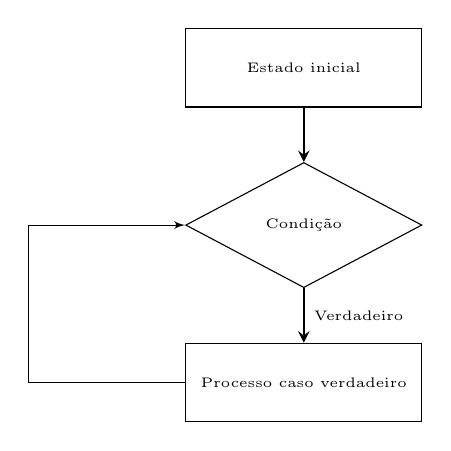
\begin{tikzpicture}[node distance=2cm]
   \node (s) [process] {\tiny Estado inicial};
   \node (d) [decision, below of=s] {\tiny Condição};
   \node (t) [process, below of=d] {\tiny Processo caso verdadeiro};
   \draw [arrow] (s) -- (d);
   \draw [arrow] (d) -- node[anchor=west] {\tiny Verdadeiro} (t);
   \path [line] (t) -- ++(-3.5,0) |- (d);
   \end{tikzpicture}
\end{minipage}
\begin{minipage}[b]{0.45\linewidth}\centering
\begin{lstlisting}[style=pseudo]
para estado_inicial ate condição
   Processo_caso_verdadeiro()
fim para
\end{lstlisting}
\end{minipage}




\begin{center} Subrotina \end{center}
\begin{minipage}[b]{0.45\linewidth}\centering
   Fluxograma\_subrotina \\
   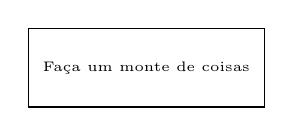
\begin{tikzpicture}[node distance=2cm]
   \node (null) [process] {\tiny Faça um monte de coisas};
   \end{tikzpicture}\\
   Seu programa\\
   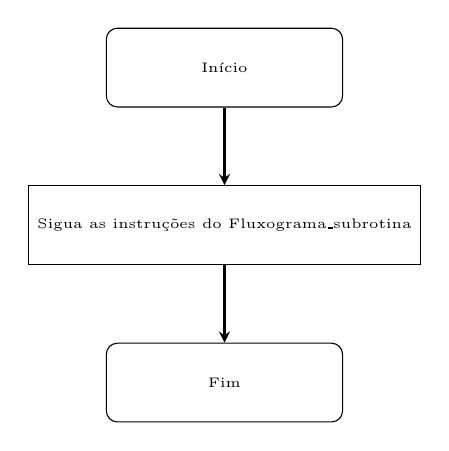
\begin{tikzpicture}[node distance=2cm]
   \node (start) [startstop] {\tiny Início};
   \node (proc) [process, below of=start] {\tiny Sigua as instruções do Fluxograma\_subrotina};
   \node (stop) [startstop, below of=proc] {\tiny Fim};
   \draw [arrow] (start) -- (proc);
   \draw [arrow] (proc) -- (stop);
   \end{tikzpicture}
\end{minipage}
\begin{minipage}[b]{0.45\linewidth}\centering
\begin{lstlisting}[style=pseudo]
subrotina foo
   Faça um monte de coisas
fim foo

inicio
   foo()
fim
\end{lstlisting}
\end{minipage}




\begin{center} Função \end{center}
\begin{minipage}[b]{0.45\linewidth}\centering
   $f(x)$ \\
   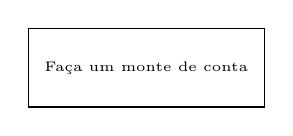
\begin{tikzpicture}[node distance=2cm]
   \node (null) [process] {\tiny Faça um monte de conta};
   \end{tikzpicture}\\
   Programa \\
   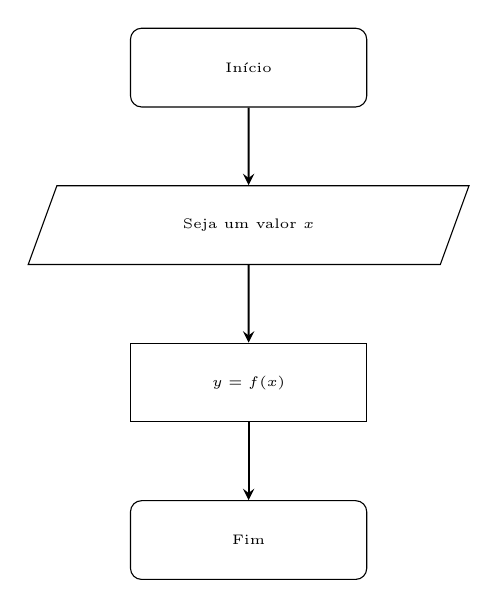
\begin{tikzpicture}[node distance=2cm]
   \node (start) [startstop] {\tiny Início};
   \node (x) [io, below of=start] {\tiny Seja um valor $x$ };
   \node (proc) [process, below of=x] {\tiny $y = f(x)$ };
   \node (stop) [startstop, below of=proc] {\tiny Fim};
   \draw [arrow] (start) -- (x);
   \draw [arrow] (x) -- (proc);
   \draw [arrow] (proc) -- (stop);
   \end{tikzpicture}
\end{minipage}
\begin{minipage}[b]{0.45\linewidth}\centering
\begin{lstlisting}[style=pseudo]
funcao f(x)
   f ← Um monte de conta
fim f

inicio
   variavel x, imagem
   x ← algum valor
   imagem ← f(x)
fim
\end{lstlisting}
\end{minipage}






Por exemplo, o pseudocódigo para calcular o fatorial é como mostrado abaixo.

\begin{lstlisting}[style=pseudo]
inicio
   escrever("Digite um número inteiro")
   ler(n)
   fatorial ← 1
   para i ← 2 ate i=n
      fatorial ← fatorial * i
      i ← i+1
   fim para
   escrever("O fatorial de " n " é " fatorial)
fim
\end{lstlisting}

\noindent
Ou, colocando tudo e só o que tem a ver com o fatorial em uma função.

\begin{lstlisting}[style=pseudo]
funcao fatorial(n)
   tmp ← 1
   para i ← 2 ate i=n
      tmp ← tmp * i
      i ← i+1
   fim para
   fatorial ← tmp
fim fatorial

inicio
   escrever("Digite um número inteiro")
   ler(n)
   escrever("O fatorial de " n " é " fatorial(n))
fim
\end{lstlisting}

\noindent
Esse método de calcular o fatorial é o método iterativo, o método recursivo
é ainda mais simples de implementar.

\begin{lstlisting}[style=pseudo]
funcao fatorial(n)
   se n > 1 entao
      fatorial ← n * fatorial(n-1)
   senao
      fatorial ← 1
   fim se
fim fatorial

inicio
   escrever("Digite um número inteiro")
   ler(n)
   escrever("O fatorial de " n " é " fatorial(n))
fim
\end{lstlisting}


\section{Material Complementar}

\begin{enumerate}[nosep]
   \item \bibentry{OqueeotaldoAlgoritmo}
   \item \bibentry{ALGORITMOSDEORDENACAO}
   \item \bibentry{OPROBLEMADOCAIXEIROVIAJANTE}
   \item \bibentry{OPODERDARECURSIVIDADE}
   \item \bibentry{RECURSIVIDADEEMACAO}
   \item \bibentry{CursodeLogicadeProgramacao}
\end{enumerate}

% %%%%%%%%%%%%%%%%%%%%%%%%%%%%%%%%%%%%%%%%%%%%%%%%%%%%%%%%%%%%%%%%%%%%%%%%%%%%%%
% Alguns Algoritmos
% %%%%%%%%%%%%%%%%%%%%%%%%%%%%%%%%%%%%%%%%%%%%%%%%%%%%%%%%%%%%%%%%%%%%%%%%%%%%%%
\chapter{Alguns Algoritmos}

\lettrine{A}{gora} que aprendemos o que são e qual a utilidade dos algoritmos,
é bastante conveniente entender alguns algoritmos. Irei apresentar algoritmos
famosos que podem ser implementados em qualquer linguagem de programação,
de fato no próximo capítulo irei apresentar uma implementação de cada
algoritmo mostrado aqui em cada linguagem de programação
(serão quatro algoritmos e quatro linguagens).

Os algoritmos serão apresentados em pseudocódigo o que já sugere como
implementar em algum programa, além de forçar o aluno a entender, pelo menos,
o pseudocódigo.

Uma dica que dou, se você escolhe aprender Fortran, por exemplo,
e nos seus estudos consegue entender o meu programa para implementar o
Crivo de Eratóstenes, é interessante tentar implementar também os outros
algorítmos que irei mostrar.





\section{Algoritmo de Euclides}

Sejam dois números naturais diferentes de zero, se pergunta:
\textit{Qual o maior divisor comum (MDC) entre eles?}

O Algoritmo de Euclides é uma maneira de responder essa pergunta
de maneira simples e eficaz, sem usar qualquer fatoração (como, creio, aprendemos na escola).
O registro mais antigo do uso desse algoritmo é da obra
\textit{Elementos}, por volta de 300 a.C., do matemático grego Euclides de Alexandria (300 a.C.),
o que faz dele um dos algoritmos mais
antigos ainda em uso.

O Algoritmo é baseado no fato de que
\[
\operatorname{MDC}(a, b) =
\left\{
\begin{aligned}
a & \text{~se~} b = 0 \\
\operatorname{MDC}(b, r) & \text{~se~} b \neq 0 \text{~e~} b < a
\end{aligned}\right.
\]

\noindent
Onde $r$ é o resto da divisão inteira $\frac{a}{b}$.
Note que, na divisão inteira $q = \frac{a}{b}$ temos que
$r = a - b q$.

\begin{lstlisting}[style=pseudo]
funcao MDC(inteiro a, inteiro b) // Considerando b < a

   se b = 0 entao
      MDC ← a
   senao
      inteiro r
      r ← a - b * (a / b)
      MDC ← MDC(b, r)
   fim se
      
fim MDC
\end{lstlisting}

Note que esta é uma definição recursiva do MDC. A partir dela podemos obter
a versão iterativa notando que o primeiro argumento sempre é trocado pelo
segundo e o segundo sempre é trocado pelo resto antes da próxima iteração.

\begin{lstlisting}[style=pseudo]
funcao MDC(inteiro a, inteiro b) // Considerando b < a

   enquanto b != 0
      r ← a - b * (a / b)
      a ← b
      b ← r
   fim enquanto
   MDC ← a
      
fim MDC
\end{lstlisting}

Os algoritmos recursivos são muito interessantes pela sua simplicidade, também
acredito que são mais fáceis de entender. Entretanto, recomendo que
sempre que possível implemente a versão iterativa do algoritmo.





\section{O Crivo de Eratóstenes}

Seja um inteiro positivo $n$, se pergunta: \textit{Quais são todos
os números primos menores ou iguais a $n$?}

O algoritmo mais famoso para resolver esse problema é atribuído
ao matemático grego Eratóstenes de Cirene (285-194 a.C.) na obra
\textit{Introdução à Aritmética} do também grego Nicómaco de Gerasa (60-120 d.C.).

O Crivo de Eratóstenes consiste em escrever uma lista de todos os números inteiros
de 2 até $n$, aceitar que 2 é primo e riscar da lista todos os números múltiplos
de 2 e maiores que 2, aceitar que o próximo número não riscado $p_2$ é primo
e riscar todos os múltiplos de $p_2$ maiores que $p_2$, ..., aceitar
que o próximo número não riscado $p_i$ é primo e riscar todos os
múltiplos de $p_i$ maiores que $p_i$, ..., e assim até que não restem números
para riscar.

\begin{lstlisting}[style=pseudo]
subrotina crivo_de_eratostenes(inteiro n)

   lista[n] // Lista com n elementos

   para i ← 2 ate n
      lista[i] = i // Escrevendo a lista
      i ← i + 1
   fim para

   para i ← 2 ate n
      se lista[i] não está riscado entao
         lista[i] é primo
         para j ← i + i ate n // Ciclo para riscar os números não primos
            riscar lista[i]
            j ← j + i
         fim para
      fim se
      i ← i + 1
   fim para
      
fim crivo_de_eratostenes
\end{lstlisting}





\section{Sequência de Fibonacci}

A sequência atribuída ao italiano Leonardo Fibonacci (1170-1250 d.C.)
é uma sequência onde os termos são a soma dos dois
números precedentes, a sequência geralmente é iniciada com
1 e 1. Em termos recursivos podemos definir os números da sequência
como sendo tais que

\[
\begin{aligned}
F_1 &= 1 \\
F_2 &= 1 \\
F_i &= F_{i-1} + F_{i-2} ~\forall~i \ge 3
\end{aligned}
\]

\begin{lstlisting}[style=pseudo]
subrotina sequencia_de_fibonacci(inteiro n)

   numero_menos1 ← 1
   numero_menos2 ← 1

   escrever("A Sequencia de Fibonacci é:")
   escrever(numero_menos1)
   escrever(numero_menos2)

   para i ← 3 ate n
      numero ← numero_menos1 + numero_menos2
      escrever(numero)
      numero_menos2 ← numero_menos1
      numero_menos1 ← numero
      i ← i + 1
   fim para
      
fim crivo_de_eratostenes
\end{lstlisting}





\section{Torre de Hanói}

Se diz que no centro do universo há um templo Hindu onde Brama haveria
colocado uma torre com 64 discos de ouro, de raios todos diferentes, e mais duas torres sem discos.
Brama ordenou que todos os dias os monges trocassem um disco de torre sem
colocar um disco maior sobre um menor. Quando todos os discos estiverem em uma
torre diferente então o templo desmoronaria e o mundo desapareceria.

O problema foi desenvolvido pelo matemático francês Édouard Lucas (1842-1891 d.C.),
consiste em obter uma sucessão de passos para mover todos os discos de torre
e ficou conhecido como problema da Torre de Hanói. Vamos considerar o problema
com $n$ discos a desenvolver a solução recursiva apresentada pela Inês. \cite{RECURSIVIDADEEMACAO}
Para tanto considere que todos os $n$ discos se encontram no pilar inicial,
que chamaremos de \texttt{ini}, que queremos mover todos para o pilar
final \texttt{fin} e que o outro pilar é o auxiliar \texttt{aux}.

Represente por \texttt{ini -> fin} o ato de mover um disco da torre inicial
para a torre final, etc.

Para o caso onde $n=2$ a solução é simples, a saber
\texttt{ini -> aux, ini -> fin, aux -> fin}.

Note que para mover $n$ discos para o pilar final
basta saber mover $n-1$ discos, dessa forma:
\begin{enumerate}[nosep]
\item Movemos os $n-1$ discos
para a torre auxiliar;
\item Movemos o maior disco para o pilar final; e
\item Voltamos a mover os $n-1$ discos para o pilar final.
\end{enumerate}

\begin{lstlisting}[style=pseudo]
funcao torre_de_hanoi(n_discos, ini, aux, fin)

   se n_discos > 0 entao
      torre_de_hanoi(n_discos-1, ini, fin, aux)
      escreva(ini "->" fin)
      torre_de_hanoi(n_discos-1, aux, ini, fin)
   fim se

fim torre_de_hanoi
\end{lstlisting}





\section{Material Complementar}

\begin{enumerate}[nosep]
\item \bibentry{AlgoritmodeEuclides}
\item \bibentry{CrivodeEratostenes}
\item \bibentry{ComoencontrarnumerosprimosoCrivodeEratostenes}
\item \bibentry{SequenciadeFibonacci}
\item \bibentry{ASEQUENCIADEFIBONACCI}
\item \bibentry{TorredeHanoi}
\item \bibentry{RECURSIVIDADEEMACAO}
\end{enumerate}

% %%%%%%%%%%%%%%%%%%%%%%%%%%%%%%%%%%%%%%%%%%%%%%%%%%%%%%%%%%%%%%%%%%%%%%%%%%%%%%
% Linguagens de programação
% %%%%%%%%%%%%%%%%%%%%%%%%%%%%%%%%%%%%%%%%%%%%%%%%%%%%%%%%%%%%%%%%%%%%%%%%%%%%%%
\chapter{Linguagens de programação}

\lettrine{C}{hegamos} ao momento de aprender a programar e implementar algoritmos.
Esse trabalho pode ser realmente difícil e exige muita dedicação, justamente
por isso recomendo que comece a estudar antes de se deparar com a matéria
no curso de Física. Para aqueles que não possuem a matéria na grade, ainda
assim é sempre de muita importância saber programar nos nossos tempos.

Usar uma linguagem de programação é como usar um pseudocódigo,
da mesma forma que escrevíamos pseudocódigo, agora vamos escrever \textbf{código
fonte} para representar as instruções que o computador deve seguir para resolver
determinado problema, as instruções devem ser ainda mais
precisas --- pois o computador é uma máquina extremamente estúpida --- e
devem seguir religiosamente as regras da linguagem escolhida para programação.
Naturalmente, a primeira tarefa é escolher uma linguagem de programação e
começar a estudar. A rigor qualquer linguagem serve e falarei de quatro linguagens,
a saber, C, Fortran, Java e Python. Quanto à sua utilidade na física recomendo o seguinte uso:
\begin{itemize}[nosep]
\item Use C ou Fortran para fazer simulações que realizam uma quantidade
astronômica de cálculos.
\item Use Java ou Python para divulgação científica ou para tratamento de dados.
\end{itemize}

Neste ponto o leitor pode escolhe uma linguagem, ou todas, e avançar para a
próxima seção. Se ainda está indeciso recomendo que estude Fortran,
que é uma linguagem feita para se usar na Física. Se quiser
aprofundar um pouco mais seus conhecimentos em ciência da computação, continue
a leitura no próximo parágrafo.

Você já notou que ao baixar alguns programas você deve escolher entre a versão
para Linux ou Windows e entre 32 ou 64bit (Firefox é um exemplo) enquanto que outros programas
precisam baixar um arquivo somente para qualquer computador (Minecraft é um exemplo)?
O primeiro tipo depende do sistema, enquanto que o segundo não e a razão disso
pode estar na linguagem que o programa é escrito.
O navegador Firefox, por exemplo, é escrito em C enquanto que o Minecraft é escrito
em Java. Mas qual a diferença?
Primeiramente note que um computador (ou máquina) é bastante estúpido e não é capaz de ler
e executar um código em nenhuma linguagem de programação.
Isso torna necessário desenvolver um programa capaz de transformar o código
em algo que o computador pode executar, há basicamente três maneiras de fazer isso:
1) O código fonte é convertido em \textbf{código objeto}, o código objeto por sua vez deve
ser algo que a máquina é capaz de executar. O programa que faz a conversão
é chamado de \textbf{compilador};
2) O código fonte é convertido em \textit{\bfseries bytecode}, o
\textit{bytecode} por sua vez só pode ser executado por um outro programa específico.
O programa que faz a conversão também é chamado de compilador
e o que executa é chamado de \textbf{Máquina Virtual};
3) O código fonte é interpretado e executado sem que o usuário tenha que se preocupar
em como a máquina se torna capaz de executar o programa.
O programa que interpreta é chamado de \textbf{intérprete}.

C e Fortran são representantes do grupo cujo o produto da compilação é
o código objeto. Esse tipo de compilação costuma gerar instruções em bytes
de procedimentos que devem ser seguidos pelo processador, claro está que
sistemas e processadores diferentes não reconhecerão o mesmo código objeto,
de maneira que o código fonte deve ser compartilhado entre as máquinas
e recompilado. A vantagem desse tipo de abordagem é a garantia de que as
instruções do código objeto são feitas especificamente para seu processador, otimizando
assim seu programa.
Java é nosso representante do grupo cujo o produto da compilação é um \textit{bytecode}.
As instruções em bytes geradas nesse tipo de compilação não podem ser diretamente
executadas pelo processador, a Máquina Virtual Java (JVM) é quem executa as instruções,
dessa forma um único \textit{bytecode} pode ser executado em qualquer máquina
que possua uma JVM instalada.
A vantagem desse tipo de abordagem é que fica mais simples de compartilhar o
executável e exije menos conhecimento do usuário final para executar,
o que torna o Java uma boa ideia para compartilhar programas de divulgação
ou pequenos aplicativos. A desvantagem é a necessidade da JVM como intermediário,
o que pode prejudicar a eficiência do programa.
Já o Python representa o grupo que não precisa ser compilado.
Programas assim podem ser facilmente compartilhados e executados em máquinas
diferentes, o que faz do Python ótimo para desenvolver programas de divulgação.
As funções disponíveis nas bibliotecas do Python também são ótimas para a
análise de dados.

Para o uso na física nós iremos querer utilizar algumas funções pré-implementadas
--- como seno e raiz quadrada, por exemplo --- e todas as linguagens de que falei
as possuem de maneira padrão, ou seja, o usuário não precisa implementar as principais funções
matemáticas, basta usar. Entretanto a experiência mostra que as implementações
do C e do Fortran costumam ser deveras mais eficientes que as do Python,
outro fator contra o Python é que sua filosofia de programação pode exigir
muitas operações que não seriam feitas em um programa equivalente em C ou Fortran,
este último contratempo também pode ser encontrado no Fortran em relação ao C.

Nas seções seguintes irei comentar algumas características de cada linguagem,
apresentar o programa \aspas{Olá Mundo}, e um exemplo de implementação de um dos
algoritmos citados no capítulo anterior. Este não é um curso de programação
e não entrarei em muitos detalhes básicos mas irei fornecer bons tutoriais na internet
que espero que lhes sejam úteis.





\section{C}

{\centering\ttfamily ola\_mundo.c}
\lstinputlisting[style=c]{programas/ola_mundo.c}

{\centering Tutoriais}
\begin{enumerate}[nosep]
\item \bibentry{CursodedeC}
\item \bibentry{LinguagemC}
\item \bibentry{LinguagemCbook}
\end{enumerate}

\begin{center} if \end{center}
\begin{minipage}[b]{0.45\linewidth}\centering
   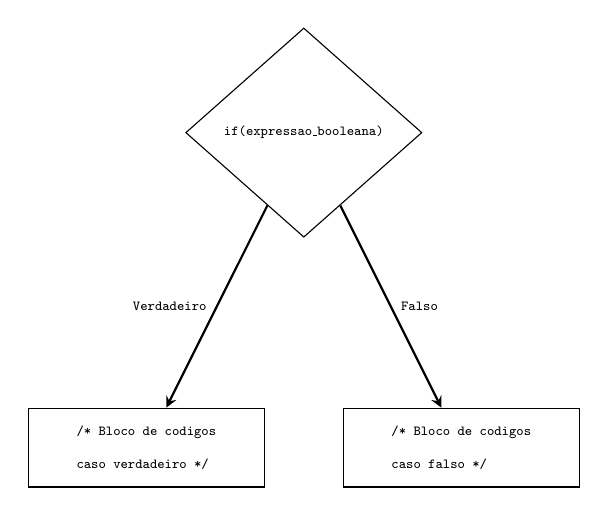
\begin{tikzpicture}[node distance=4cm]
   \node (d) [decision] {\tiny\ttfamily if(expressao\_booleana)};
   \node (t) [process, below of=d, xshift=-2cm, align=left] {\tiny\ttfamily /* Bloco de codigos\\\tiny\ttfamily caso verdadeiro */};
   \node (f) [process, below of=d, xshift=2cm, align=left] {\tiny\ttfamily /* Bloco de codigos\\\tiny\ttfamily caso falso */};
   \draw [arrow] (d) -- node[anchor=east] {\tiny\ttfamily Verdadeiro} (t);
   \draw [arrow] (d) -- node[anchor=west] {\tiny\ttfamily Falso} (f);
   \end{tikzpicture}
\end{minipage}
\begin{minipage}[b]{0.45\linewidth}\centering
\begin{lstlisting}[style=c]
if(expressao_booleana){
   /* Bloco de codigos caso verdadeiro */
}else{
   /* Bloco de codigos caso falso */
}
\end{lstlisting}
\end{minipage}

\begin{center} while \end{center}
\begin{minipage}[b]{0.45\linewidth}\centering
   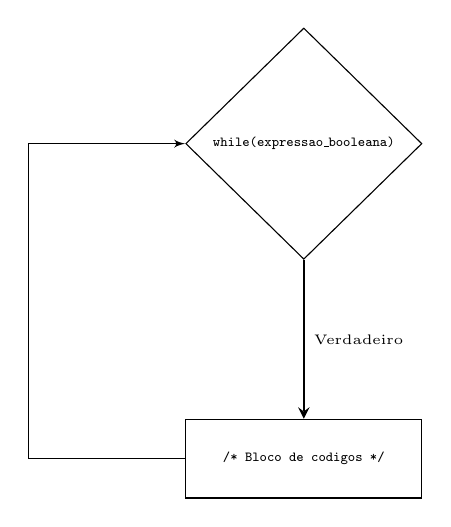
\begin{tikzpicture}[node distance=4cm]
   \node (d) [decision] {\tiny\ttfamily while(expressao\_booleana)};
   \node (t) [process, below of=d] {\tiny\ttfamily /* Bloco de codigos */};
   \draw [arrow] (d) -- node[anchor=west] {\tiny Verdadeiro} (t);
   \path [line] (t) -- ++(-3.5,0) |- (d);
   \end{tikzpicture}
\end{minipage}
\begin{minipage}[b]{0.45\linewidth}\centering
\begin{lstlisting}[style=c]
while(expressao_booleana){
   /* Bloco de codigos */
}
\end{lstlisting}
\end{minipage}

\begin{center} for \end{center}
\begin{minipage}[b]{0.45\linewidth}\centering
   \begin{tikzpicture}[node distance=3cm]
   \node (s) [process] {\tiny\ttfamily inicio};
   \node (d) [decision, below of=s] {\tiny\ttfamily expressao\_booleana};
   \node (t) [process, below of=d] {\tiny\ttfamily /* Bloco de codigos */};
   \node (i) [process, below of=t] {\tiny\ttfamily inclemento};
   \draw [arrow] (s) -- (d);
   \draw [arrow] (d) -- node[anchor=west] {\tiny\ttfamily Verdadeiro} (t);
   \draw [arrow] (t) -- (i);
   \path [line] (i) -- ++(-3.5,0) |- (d);
   \end{tikzpicture}
\end{minipage}
\begin{minipage}[b]{0.45\linewidth}\centering
\begin{lstlisting}[style=c]
for(inicio; expressao_booleana; inclemento){
   /* Bloco de codigos */
}
\end{lstlisting}
\end{minipage}

\begin{center} Cabeçalho \end{center}
\begin{lstlisting}[style=c]
#include <stdio.h> /* Para manusear arquivos */
#include <math.h> /* Para usar funcoes matematicas */
\end{lstlisting}

\newpage
{\centering\ttfamily mdc.c}
\lstinputlisting[style=c]{programas/mdc.c}
\newpage




\section{Fortran}

{\centering\ttfamily ola\_mundo.f90}
\lstinputlisting[style=f90]{programas/ola_mundo.f90}

{\centering Tutoriais}
\begin{enumerate}[nosep]
\item \bibentry{CursodeFortran90}
\item \bibentry{CursodeFortran}
\item \bibentry{IntroducaoFortran}
\end{enumerate}

\begin{center} IF \end{center}
\begin{minipage}[b]{0.45\linewidth}\centering
   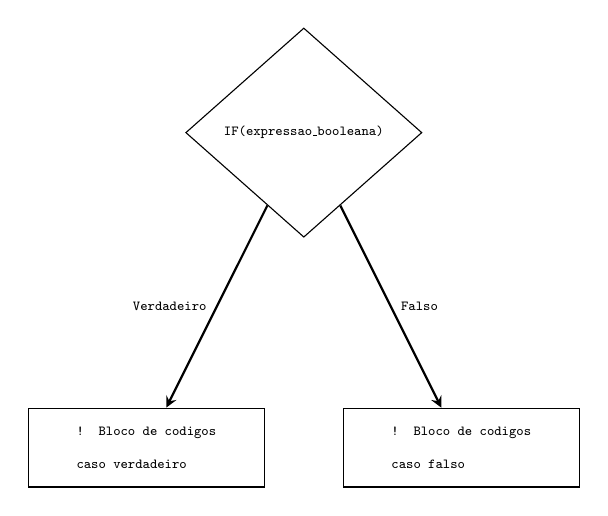
\begin{tikzpicture}[node distance=4cm]
   \node (d) [decision] {\tiny\ttfamily IF(expressao\_booleana)};
   \node (t) [process, below of=d, xshift=-2cm, align=left] {\tiny\ttfamily ! Bloco de codigos\\\tiny\ttfamily caso verdadeiro};
   \node (f) [process, below of=d, xshift=2cm, align=left] {\tiny\ttfamily ! Bloco de codigos\\\tiny\ttfamily caso falso};
   \draw [arrow] (d) -- node[anchor=east] {\tiny\ttfamily Verdadeiro} (t);
   \draw [arrow] (d) -- node[anchor=west] {\tiny\ttfamily Falso} (f);
   \end{tikzpicture}
\end{minipage}
\begin{minipage}[b]{0.45\linewidth}\centering
\begin{lstlisting}[style=f90]
IF(expressao_booleana) THEN
   ! Bloco de codigos caso verdadeiro
ELSE
   ! Bloco de codigos caso falso
END IF
\end{lstlisting}
\end{minipage}

\begin{center} DO \end{center}
\begin{minipage}[b]{0.45\linewidth}\centering
   \begin{tikzpicture}[node distance=3cm]
   \node (s) [process] {\tiny\ttfamily inicio};
   \node (d) [decision, below of=s] {\tiny\ttfamily expressao\_booleana};
   \node (t) [process, below of=d] {\tiny\ttfamily ! Bloco de codigos};
   \node (i) [process, below of=t] {\tiny\ttfamily inclemento};
   \draw [arrow] (s) -- (d);
   \draw [arrow] (d) -- node[anchor=west] {\tiny\ttfamily Verdadeiro} (t);
   \draw [arrow] (t) -- (i);
   \path [line] (i) -- ++(-3.5,0) |- (d);
   \end{tikzpicture}
\end{minipage}
\begin{minipage}[b]{0.45\linewidth}\centering
\begin{lstlisting}[style=f90]
DO inicio, expressao_booleana, inclemento
   ! Bloco de codigos
END DO
\end{lstlisting}
\end{minipage}

\begin{center}do  while \end{center}
\begin{minipage}[b]{0.45\linewidth}\centering
   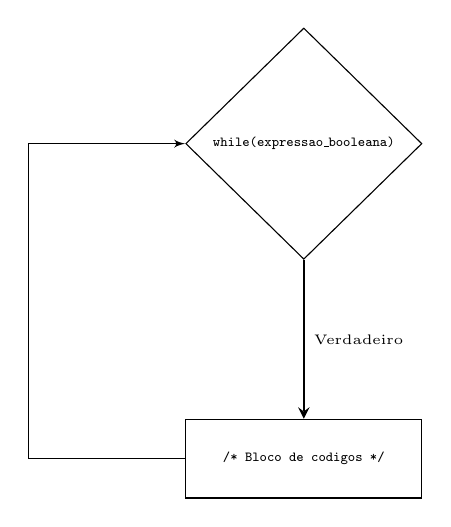
\begin{tikzpicture}[node distance=4cm]
   \node (d) [decision] {\tiny\ttfamily while(expressao\_booleana)};
   \node (t) [process, below of=d] {\tiny\ttfamily /* Bloco de codigos */};
   \draw [arrow] (d) -- node[anchor=west] {\tiny Verdadeiro} (t);
   \path [line] (t) -- ++(-3.5,0) |- (d);
   \end{tikzpicture}
\end{minipage}
\begin{minipage}[b]{0.45\linewidth}\centering
\begin{lstlisting}[style=f90]
DO WHILE (expressao_booleana)
   ! Bloco de codigos
END DO
\end{lstlisting}
\end{minipage}

\newpage
{\centering\ttfamily crivo.f90}
\lstinputlisting[style=f90]{programas/crivo.f90}
\newpage




\section{Java}

{\centering\ttfamily ola\_mundo.java}
\lstinputlisting[style=java]{programas/ola_mundo.java}

{\centering Tutoriais}
\begin{enumerate}[nosep]
\item \bibentry{CursodeJava}
\item \bibentry{MaratonaJava}
\item \bibentry{ALINGUAGEMDEPROGRAMACAOJAVA}
\end{enumerate}

\begin{center} if \end{center}
\begin{minipage}[b]{0.45\linewidth}\centering
   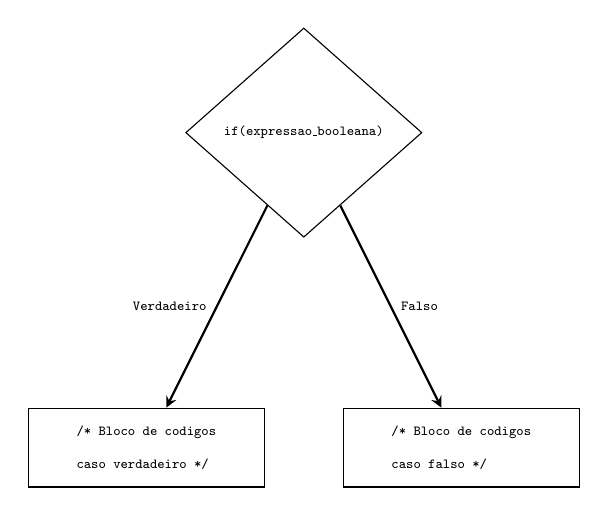
\begin{tikzpicture}[node distance=4cm]
   \node (d) [decision] {\tiny\ttfamily if(expressao\_booleana)};
   \node (t) [process, below of=d, xshift=-2cm, align=left] {\tiny\ttfamily /* Bloco de codigos\\\tiny\ttfamily caso verdadeiro */};
   \node (f) [process, below of=d, xshift=2cm, align=left] {\tiny\ttfamily /* Bloco de codigos\\\tiny\ttfamily caso falso */};
   \draw [arrow] (d) -- node[anchor=east] {\tiny\ttfamily Verdadeiro} (t);
   \draw [arrow] (d) -- node[anchor=west] {\tiny\ttfamily Falso} (f);
   \end{tikzpicture}
\end{minipage}
\begin{minipage}[b]{0.45\linewidth}\centering
\begin{lstlisting}[style=java]
if(expressao_booleana){
   /* Bloco de codigos caso verdadeiro */
}else{
   /* Bloco de codigos caso falso */
}
\end{lstlisting}
\end{minipage}

\begin{center} while \end{center}
\begin{minipage}[b]{0.45\linewidth}\centering
   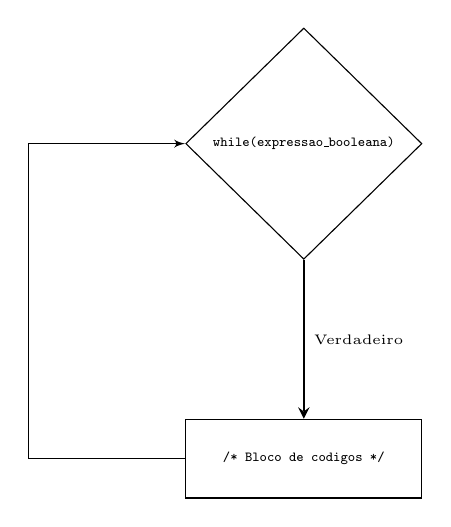
\begin{tikzpicture}[node distance=4cm]
   \node (d) [decision] {\tiny\ttfamily while(expressao\_booleana)};
   \node (t) [process, below of=d] {\tiny\ttfamily /* Bloco de codigos */};
   \draw [arrow] (d) -- node[anchor=west] {\tiny Verdadeiro} (t);
   \path [line] (t) -- ++(-3.5,0) |- (d);
   \end{tikzpicture}
\end{minipage}
\begin{minipage}[b]{0.45\linewidth}\centering
\begin{lstlisting}[style=java]
while(expressao_booleana){
   /* Bloco de codigos */
}
\end{lstlisting}
\end{minipage}

\begin{center} for \end{center}
\begin{minipage}[b]{0.45\linewidth}\centering
   \begin{tikzpicture}[node distance=3cm]
   \node (s) [process] {\tiny\ttfamily inicio};
   \node (d) [decision, below of=s] {\tiny\ttfamily expressao\_booleana};
   \node (t) [process, below of=d] {\tiny\ttfamily /* Bloco de codigos */};
   \node (i) [process, below of=t] {\tiny\ttfamily inclemento};
   \draw [arrow] (s) -- (d);
   \draw [arrow] (d) -- node[anchor=west] {\tiny\ttfamily Verdadeiro} (t);
   \draw [arrow] (t) -- (i);
   \path [line] (i) -- ++(-3.5,0) |- (d);
   \end{tikzpicture}
\end{minipage}
\begin{minipage}[b]{0.45\linewidth}\centering
\begin{lstlisting}[style=java]
for(inicio; expressao_booleana; inclemento){
   /* Bloco de codigos */
}
\end{lstlisting}
\end{minipage}

\newpage
{\centering\ttfamily fibonacci.java}
\lstinputlisting[style=java]{programas/fibonacci.java}
\newpage




\section{Python}

{\centering\ttfamily ola\_mundo.py}
\lstinputlisting[style=py]{programas/ola_mundo.py}

{\centering Tutoriais}
\begin{enumerate}[nosep]
\item \bibentry{CursodePython1}
\item \bibentry{CursodePython2}
\item \bibentry{CursodePython3}
\end{enumerate}

\begin{center} if \end{center}
\begin{minipage}[b]{0.45\linewidth}\centering
   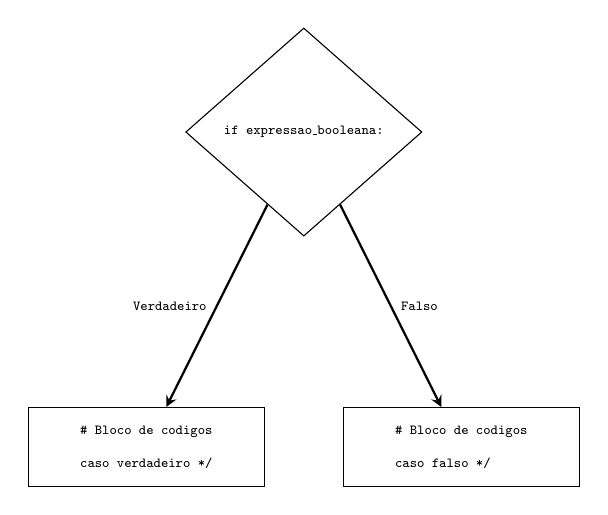
\begin{tikzpicture}[node distance=4cm]
   \node (d) [decision] {\tiny\ttfamily if expressao\_booleana:};
   \node (t) [process, below of=d, xshift=-2cm, align=left] {\tiny\ttfamily \# Bloco de codigos\\\tiny\ttfamily caso verdadeiro */};
   \node (f) [process, below of=d, xshift=2cm, align=left] {\tiny\ttfamily \# Bloco de codigos\\\tiny\ttfamily caso falso */};
   \draw [arrow] (d) -- node[anchor=east] {\tiny\ttfamily Verdadeiro} (t);
   \draw [arrow] (d) -- node[anchor=west] {\tiny\ttfamily Falso} (f);
   \end{tikzpicture}
\end{minipage}
\begin{minipage}[b]{0.45\linewidth}\centering
\begin{lstlisting}[style=py]
if expressao_booleana:
   # Bloco de codigos caso verdadeiro
else:
   # Bloco de codigos caso falso
\end{lstlisting}
\end{minipage}

\begin{center} while \end{center}
\begin{minipage}[b]{0.45\linewidth}\centering
   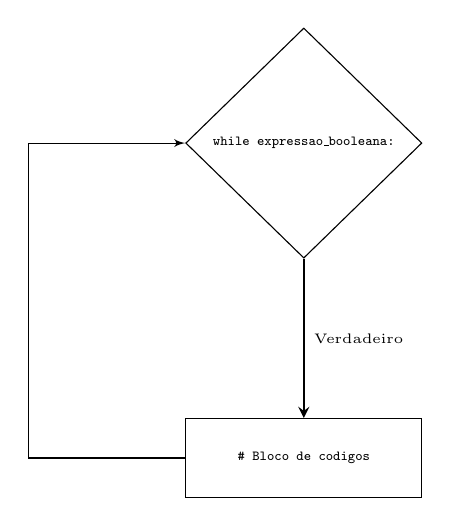
\begin{tikzpicture}[node distance=4cm]
   \node (d) [decision] {\tiny\ttfamily while expressao\_booleana:};
   \node (t) [process, below of=d] {\tiny\ttfamily \# Bloco de codigos};
   \draw [arrow] (d) -- node[anchor=west] {\tiny Verdadeiro} (t);
   \path [line] (t) -- ++(-3.5,0) |- (d);
   \end{tikzpicture}
\end{minipage}
\begin{minipage}[b]{0.45\linewidth}\centering
\begin{lstlisting}[style=py]
while expressao_booleana:
   # Bloco de codigos
\end{lstlisting}
\end{minipage}

\newpage
{\centering\ttfamily hanoi.py}
\lstinputlisting[style=py]{programas/hanoi.py}
\newpage

\section{Material Complementar}

\begin{enumerate}[nosep]
\item \bibentry{FisicaComputacional1}
\item \bibentry{FisicaComputacional2}
\end{enumerate}




% ------------------------------------------------------------------------------
% ELEMENTOS PÓS-TEXTUAIS
% ------------------------------------------------------------------------------
   \postextual

   % ---------------------------------------------------------------------------
   % Referências bibliográficas
   % ---------------------------------------------------------------------------
   \bibliography{../reference.bib}
   \appendix
   % %%%%%%%%%%%%%%%%%%%%%%%%%%%%%%%%%%%%%%%%%%%%%%%%%%%%%%%%%%%%%%%%%%%%%%%%%%%%%%
% Linux
% %%%%%%%%%%%%%%%%%%%%%%%%%%%%%%%%%%%%%%%%%%%%%%%%%%%%%%%%%%%%%%%%%%%%%%%%%%%%%%
\chapter{Instalando C, Fortran, Java e/ou Python no Linux}

\lettrine{P}{ara} instalar os compiladores de C, Fortran e Java, bem como a JVM
e o intérprete de Python
no Debian e derivados, como Ubuntu, Linux Mint, etc basta digitar
o comando abaixo no terminal.
\begin{lstlisting}[style=bash]
apt update && apt install -y gcc gfortran openjdk-17-jdk python3
\end{lstlisting}

% %%%%%%%%%%%%%%%%%%%%%%%%%%%%%%%%%%%%%%%%%%%%%%%%%%%%%%%%%%%%%%%%%%%%%%%%%%%%%%
% Android
% %%%%%%%%%%%%%%%%%%%%%%%%%%%%%%%%%%%%%%%%%%%%%%%%%%%%%%%%%%%%%%%%%%%%%%%%%%%%%%
\chapter{Instalando C, Fortran, Java e/ou Python no Android}

\lettrine{A}{} primeira coisa que vamos precisar para programar pelo
telefone é de um terminal e o melhor que há é o Termux
que pode ser baixado em
\url{https://f-droid.org/packages/com.termux/}. Após baixar e instalar o Termux
abra ele e digite as seguintes linhas de comando (tecle enter depois de cada uma).
\begin{lstlisting}[style=bash]
apt update
apt install -y wget gnupg
wget -O - cctools.info/public.key | apt-key add -
echo "deb https://cctools.info termux cctools" >\
$PREFIX/etc/apt/sources.list.d/cctools.list
\end{lstlisting}

Finalmente, para
instalar os compiladores de C, Fortran e Java, bem como a JVM
e o intérprete de Python
no Android basta digitar
o comando abaixo.
\begin{lstlisting}[style=bash]
apt update && apt install -y gcc-cctools openjdk-17 python
\end{lstlisting}

Para facilitar o uso do \texttt{gfortran} digite o
seguinte comando no terminal.
\begin{lstlisting}[style=bash]
ln -s ~/../cctools-toolchain/bin/gfortran $PREFIX/bin/gfortran
\end{lstlisting}


% %%%%%%%%%%%%%%%%%%%%%%%%%%%%%%%%%%%%%%%%%%%%%%%%%%%%%%%%%%%%%%%%%%%%%%%%%%%%%%
% Windows
% %%%%%%%%%%%%%%%%%%%%%%%%%%%%%%%%%%%%%%%%%%%%%%%%%%%%%%%%%%%%%%%%%%%%%%%%%%%%%%
\chapter{Instalando C, Fortran, Java e/ou Python no Windows}

\lettrine{B}{aixe} o instalador do OpenJDK (implementação gratis e de código aberto do java)
em
\url{https://docs.microsoft.com/pt-br/java/openjdk/download}
(procure pelo arquivo de extensão \texttt{msi})
e execute ele, certifique-se de marcar a opção \textit{Add to PATH} na
janela \textit{Custom Setup}.

Baixe o instalador do Python em
\url{https://www.python.org/downloads/release/python-3100/}
e execute ele, lembre-se de marcar a opção \textit{Add Python 3.10 to PATH}
antes de começar a instalação.
Na última janela pode aparecer a opção \textit{Disable path length limit},
execute-a.

Baixe o MinGW (Pacote que possui o GCC, que possui compiladores de C e Fortran)
em
\url{https://sourceforge.net/projects/mingw/}
e execute ele,
quando aparecer a janela \textit{MinGW Instalation Manager}
clique em \textit{Basic Setup} (à esquerda) e depois selecione, ao lado,
os pacotes \texttt{mingw32-base} e \texttt{mingw32-gcc-gfortran}
para serem instalados --- para fazer isso basta clicar no quadradinho e
depois em \textit{Mark for Installation} ---.
Depois vá à aba \textit{Installation} (em cima) e clique em \textit{Apply Changes}.
Uma vez concluida a instalação é preciso adicionar o MinGW ao PATH,
para isso pesquise no menu iniciar por
\texttt{exibir configurações avançadas do sistema} e clique na opção
\texttt{Variáveis de Ambiente}, procure pela variável \texttt{Path}
e clique em \texttt{editar} e depois em \texttt{Novo}
e escreva \aspas{\texttt{C:{\textbackslash}MinGW{\textbackslash}bin}}.


% %%%%%%%%%%%%%%%%%%%%%%%%%%%%%%%%%%%%%%%%%%%%%%%%%%%%%%%%%%%%%%%%%%%%%%%%%%%%%%
% Editores de texto e IDE's
% %%%%%%%%%%%%%%%%%%%%%%%%%%%%%%%%%%%%%%%%%%%%%%%%%%%%%%%%%%%%%%%%%%%%%%%%%%%%%%
\chapter{Editores de texto e IDE's}

Para escrever códigos precisamos de editores de texto, em geral
queremos editores que deixam as palavras coloridas conforme sua utilidade.

Linux:
\begin{itemize}[nosep]
\item Xed \url{https://github.com/linuxmint/xed}
\item Gedit \url{https://wiki.gnome.org/Apps/Gedit}
\end{itemize}

Android:
\begin{itemize}[nosep]
\item DroidEdit \url{https://play.google.com/store/apps/details?id=com.aor.droidedit}
\end{itemize}

Windows:
\begin{itemize}[nosep]
\item Gedit \url{https://wiki.gnome.org/Apps/Gedit}
\end{itemize}

Uma IDE nada mais é que um editor de texto que possui várias outras funções
para facilitar a escrita de códigos, em geral uma IDE é dedicada a uma
linguagem específica.

Linux:
\begin{itemize}[nosep]
\item Eclipse \url{https://www.eclipse.org/downloads/}
\item Visual Studio Code \url{https://code.visualstudio.com/download}
\item Code::Blocks (C, C++, Fortran) \url{https://www.codeblocks.org/downloads/binaries/}
\item Apache NetBeans \url{https://netbeans.apache.org/download/index.html}
\item Anjuta \url{https://anjuta.org/}
\end{itemize}

Android:
\begin{itemize}[nosep]
\item AIDE (C, Java) \url{https://play.google.com/store/apps/details?id=com.aide.ui}
\end{itemize}

Windows:
\begin{itemize}[nosep]
\item Eclipse \url{https://www.eclipse.org/downloads/}
\item Visual Studio Code \url{https://code.visualstudio.com/download}
\item Code::Blocks (C, C++, Fortran) \url{https://www.codeblocks.org/downloads/binaries/}
\item Apache NetBeans \url{https://netbeans.apache.org/download/index.html}
\end{itemize}



   \chapter{Licença}
   \begin{otherlanguage*}{english}
   \input{./LICENSE}
   \end{otherlanguage*}

\end{document}
